\documentclass[tikz, border=10pt]{standalone}
\usetikzlibrary{positioning, arrows.meta}

\begin{document}
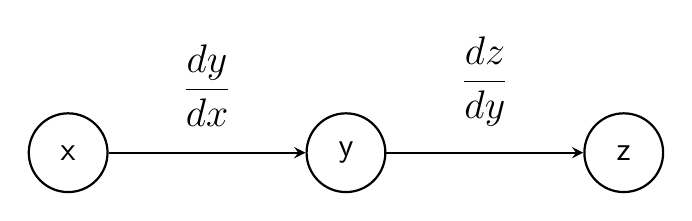
\begin{tikzpicture}[
    node distance=2.5cm,
    main node/.style={circle, draw=black, thick, minimum size=1.0cm, font=\large\sffamily},
    arrow line/.style={->, >=stealth, thick}
]

    % Nodes
    \node[main node] (x) {x};
    \node[main node] (y) [right=of x] {y};
    \node[main node] (z) [right=of y] {z};

    % Edges with labels
    \draw[arrow line] (x) -- node[above=0.2cm] {\Large $\displaystyle\frac{dy}{dx}$} (y);
    \draw[arrow line] (y) -- node[above=0.2cm] {\Large $\displaystyle\frac{dz}{dy}$} (z);

\end{tikzpicture}
\end{document}